本课程《分布式系统》指定QQ群（群号：1083024265）作为教学通知的官方发布平台。任课教师已于2026年4月3日课堂上正式宣布该安排，自宣布之日起，教师已履行教学告知义务。请全体选课学生及时加入该群并定期查阅通知；因个人未及时关注群内信息而影响作业提交或课程考核的，相关责任由学生本人承担。

\section{1 互斥：问题与基本方案}

\begin{itemize}
\item 问题：分布式系统中的多个进程需要独占访问某些资源。
\item 基本解决方案：
  \begin{itemize}
  \item 基于权限：想要进入临界区或访问资源的进程需要来自其他进程的权限。
  \item 基于令牌：令牌在进程之间传递。拥有令牌的进程可以在临界区中继续，或者在不感兴趣时传递它。
  \end{itemize}
\end{itemize}

\subsection{集中式算法}

\begin{itemize}
\item 使用协调器。
\item 协调器拥有共享资源的权限。权限被授予请求的进程。
\item 进程向协调器请求访问。
\item 如果另一个进程随后请求访问同一资源的权限，协调器不回复（直到前一个释放）。
\item 当进程释放资源时，它告诉协调器，协调器然后回复等待的下一个进程。
\end{itemize}

\subsection{Ricart \& Agrawala 算法}

与 Lamport 算法相同，除了不发送确认。

\begin{itemize}
\item 如果接收方没有访问该资源，并且也不想访问，它会向发送方发送一条 OK 消息。
\item 如果接收方已经可以访问该资源，它不会回复，而是将请求放入队列。
\item 如果接收方也想访问该资源，但尚未访问，它会将传入消息的时间戳与它发送给所有人的消息中的时间戳进行比较。时间戳较短的那个优先。
\item 如果传入消息的时间戳较短，接收方会发送一条 OK 消息；如果接收方自身的消息时间戳较短，接收方会将传入的请求放入队列，不回复。
\end{itemize}

\subsection{Ricart \& Agrawala 算法例子}

\begin{figure}[htbp]
\centering
\includegraphics[width=0.8\textwidth]{../work/figures/placeholder}
\caption{Ricart \& Agrawala 算法示例图}
\label{fig:ricart}
\end{figure}

\subsection{令牌环算法}

\begin{itemize}
\item 本质：将进程组织成逻辑环，让令牌在它们之间传递。拥有令牌的进程被允许进入临界区（如果它想的话）。构造为逻辑环的覆盖网络，带有循环令牌。
\end{itemize}

\subsection{ZooKeeper（互斥）}

\begin{itemize}
\item ZooKeeper 维护基于树的命名空间，类似于文件系统。
\item 锁定协议：客户端创建/删除节点以获取/释放锁。
\item 版本控制：用于防止竞争条件。
\end{itemize}

\section{2 选举算法}

\subsection{选举算法：原理}

\begin{itemize}
\item 许多系统要求某些进程充当协调器。问题是如何动态选择这个特殊进程。
\item 在许多系统中，协调器是手动选择的（例如集中式解决方案）。
\end{itemize}

\subsection{选举算法：基本假设}

\begin{itemize}
\item 所有进程都有唯一 ID。
\item 所有进程都知道系统中所有进程的 ID（但不知道它们是启动还是关机）。
\item 选举意味着识别启动的具有最高 ID 的进程。
\end{itemize}

\subsection{欺凌算法（Bully）}

\begin{itemize}
\item 原理：当进程注意到协调器不再响应请求时，它启动选举：Px 向所有具有更高标识符的进程发送选举消息。
\item 如果没有人响应，它赢得选举并成为协调器。
\item 如果上级之一回答，它接管，它的工作完成。
\end{itemize}

\begin{figure}[htbp]
\centering
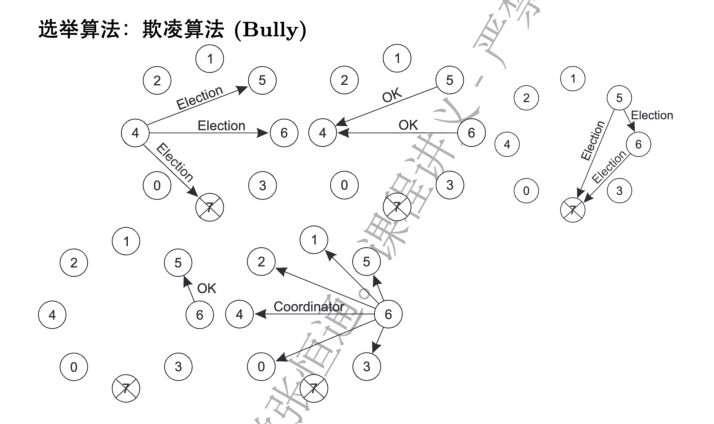
\includegraphics[width=0.8\textwidth]{figures/ch5/ch5_bully_algorithm.png}
\caption{欺凌算法示意图}
\label{fig:bully}
\end{figure}

\subsection{环算法}

\begin{itemize}
\item 基本思想：将所有进程按编号组织成一个逻辑环，通过环形传递消息完成选举。
\item 启动选举：任一进程发现协调者失效后，可主动发起选举，向环中下一位邻居发送 'Election' 消息，并附上自身编号。若下一位邻居失效，继续跳过。
\item 消息传递：每个收到 'Election' 消息的进程，将自身编号加入消息列表，继续向后转发；若消息回到发起者，说明已遍历全环，所有存活进程均已报到。
\item 确定协调者：发起者从收集到的编号中选出最大者，并广播 'Coordinator' 消息通知全体——新一轮协调者正式产生。
\end{itemize}

\begin{figure}[htbp]
\centering
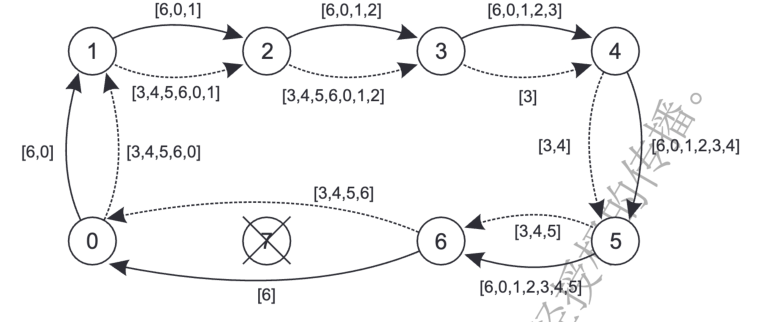
\includegraphics[width=0.8\textwidth]{figures/ch5/ch5_election_p6.png}
\caption{由 P6 发起的选举（实线）}
\label{fig:ring1}
\end{figure}

\begin{figure}[htbp]
\centering
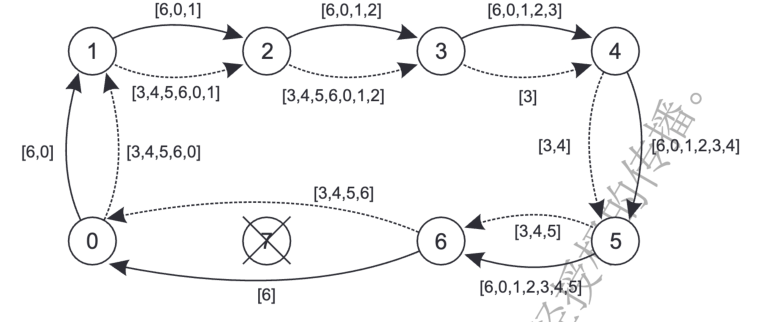
\includegraphics[width=0.8\textwidth]{figures/ch5/ch5_election_p3.png}
\caption{由 P3 发起的选举（虚线）}
\label{fig:ring2}
\end{figure}

图中实线表示由 P6 发起的选举，虚线表示 P3 发起的选举。该算法要求环结构场景。

\subsection{ZooKeeper 选举：PK 准则}

ZooKeeper 默认使用 Fast Leader Election 算法。当节点进入选举状态（LOOKING）时，遵循以下 PK 逻辑：

核心参数：
\begin{itemize}
\item ZXID (Transaction ID)：数据的新旧程度。越大的数据越新。
\item SID (Server ID)：服务器唯一编号。
\item Epoch：逻辑时钟，代表当前的选举轮次。
\end{itemize}

胜出判定（优先级由高到低）：
\begin{enumerate}
\item Epoch 优先：轮次大的直接胜出。
\item ZXID 优先：若轮次相同，数据越新的胜出。
\item SID 优先：若数据也一样新，SID 最大的胜出。
\item 注：当某个节点获得的票数超过集群总数的半数（$n/2 + 1$），即当选 Leader。
\end{enumerate}

\subsection{Fast Leader Election 算法逻辑}

每一个 ZooKeeper 节点在选举时本质上是一个状态机，其核心逻辑如下：

\begin{itemize}
\item 自增选举周期（logicalclock）：确保选举是在同一轮次进行的。
\item 初始化选票：初始状态下，每个节点都推举自己为 Leader。
\item 发送与接收：将选票广播给集群所有成员，并记录支持各投票的节点列表。
\item 收敛判定：每次更新投票后，节点统计集群中支持该投票的节点数。当某一个节点获得的票数过半，且没有更优的候选人出现时，选举终止。
\end{itemize}

状态：
\begin{itemize}
\item LOOKING：寻找 Leader 中。
\item LEADING：领导者状态。
\item FOLLOWING/OBSERVING：跟随者/观察者状态。
\end{itemize}

选举中的“见贤思齐”：为什么要改投？
在 LOOKING 状态下，每个节点都像是一个投票者。

第一阶段：自信投自己
每个节点启动时，都觉得自己是 Leader，发出一张选票：(SID, ZXID)

第二阶段：交换与动摇
收到别人的选票后，节点会进行思想斗争：
“它的数据（ZXID）比我新？”
“它的 ID 比我大？”
核心改投原则：只要对方展示出的“实力”（ZXID $>$ 我的，或 ZXID 相同但 SID 更大）比我强，我立刻撕毁旧选票，广播新选票，全心全意推举他。
结论：改投机制让选票迅速向“最强者”靠拢，实现快速收敛。

\subsection{选举流程：以5台服务器启动为例}

假设 5 台服务器 SID 分别为 1$\sim$5，按顺序启动：

\begin{table}[htbp]
\centering
\begin{tabular}{@{}ll@{}}
\toprule
启动顺序 & 选票变动与结果 \\
\midrule
Server 1 & 投自己 (1票) 票数未过半 (1/5)，等待 \\
Server 2 & Server 1 发现 2 的 SID 更大，改投 2，2号获得 2 票，未过半 \\
Server 3 & 1、2 发现 3 的 SID 最大，均改投 3，Server 3 晋升为 Leader \\
Server 4,5 & 发现已有 Leader，选举结束，直接以 Follower 身份加入 \\
\bottomrule
\end{tabular}
\caption{选举流程示例}
\label{tab:election}
\end{table}

\begin{itemize}
\item 崩溃恢复选举：当 Leader 宕机，其余节点进入 LOOKING，按上述 PK 流程重新选举。
\item 防脑裂：过半机制确保了全网只可能产生一个合法的 Leader 节点。
\end{itemize}

\subsection{经典选举与现代共识回顾}

基于 Bully 等算法：
\begin{itemize}
\item 假设：同步通信、无消息丢失、进程身份稳定；
\item 问题：一旦网络分区、消息延迟或节点反复宕机/重启，可能陷入：
  \begin{itemize}
  \item 活锁：多个进程/节点在不断尝试执行某个动作（如发起选举），但因互相干扰，导致谁都无法成功完成任务。
  \item 脑裂：系统中同时存在多个节点认为自己是协调者（Leader），并对外提供服务。
  \item 网络分区：网络故障导致集群分裂成多个子集，每个子集独立选出自己的 Leader，并继续处理请求。
  \end{itemize}
\end{itemize}

\subsection{经典选举与现代共识：现实挑战}

\begin{itemize}
\item 异步网络：消息延迟无上限（FLP 不可能性）；
\item 动态节点：节点随时加入/退出（如云环境）；
\item 状态一致性：不仅要选 Leader，更要保证状态一致！

且看：基于日志复制的共识协议（下章介绍）。
\end{itemize}

\bigskip

本次课汇报完毕。
欢迎大家批评指教。

对应课程教材第五章。
